% This file was created by tikzplotlib v0.8.5.
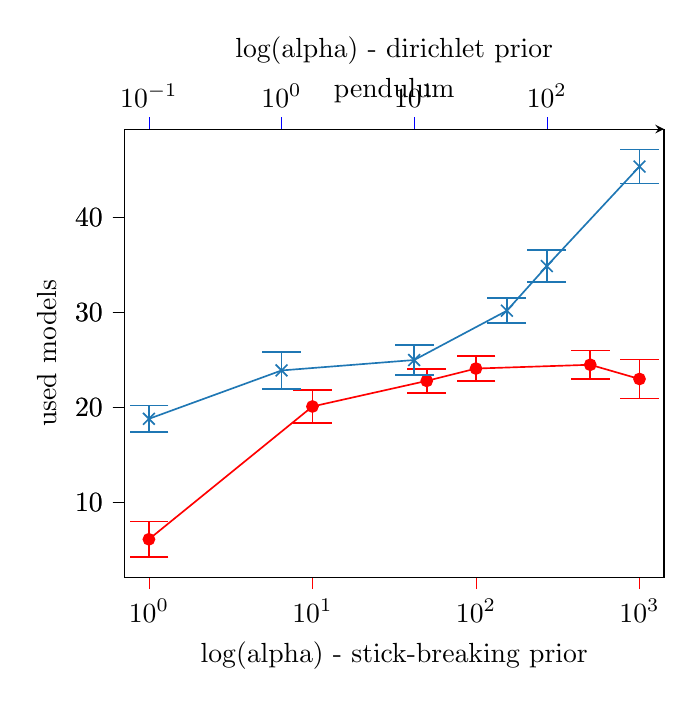
\begin{tikzpicture}

\definecolor{color0}{rgb}{0.12156862745098,0.466666666666667,0.705882352941177}

\begin{axis}[
log basis x={10},
tick align=outside,
tick pos=left,
title={pendulum},
x grid style={white!69.01960784313725!black},
xlabel={log(alpha) - stick-breaking prior},
xmin=0.707945784384138, xmax=1412.53754462275,
xmode=log,
xtick style={color=red},
xtick={0.01,0.1,1,10,100,1000,10000,100000},
xticklabels={\(\displaystyle {10^{-2}}\),\(\displaystyle {10^{-1}}\),\(\displaystyle {10^{0}}\),\(\displaystyle {10^{1}}\),\(\displaystyle {10^{2}}\),\(\displaystyle {10^{3}}\),\(\displaystyle {10^{4}}\),\(\displaystyle {10^{5}}\)},
y grid style={white!69.01960784313725!black},
ylabel={used models},
ymin=2.08343812231171, ymax=49.3484077084613,
ytick style={color=black}
]
\path [draw=red, semithick]
(axis cs:1,4.23184583077306)
--(axis cs:1,7.96815416922694);

\path [draw=red, semithick]
(axis cs:10,18.3421604168753)
--(axis cs:10,21.8578395831247);

\path [draw=red, semithick]
(axis cs:50,21.5510004003203)
--(axis cs:50,24.0489995996797);

\path [draw=red, semithick]
(axis cs:100,22.8)
--(axis cs:100,25.4);

\path [draw=red, semithick]
(axis cs:500,23)
--(axis cs:500,26);

\path [draw=red, semithick]
(axis cs:1000,20.9506098468081)
--(axis cs:1000,25.0493901531919);

\addplot [semithick, red, mark=-, mark size=7, mark options={solid}, only marks]
table {%
1 4.23184583077306
10 18.3421604168753
50 21.5510004003203
100 22.8
500 23
1000 20.9506098468081
};
\addplot [semithick, red, mark=-, mark size=7, mark options={solid}, only marks]
table {%
1 7.96815416922694
10 21.8578395831247
50 24.0489995996797
100 25.4
500 26
1000 25.0493901531919
};
\addplot [semithick, red, mark=*, mark size=2, mark options={solid}]
table {%
1 6.1
10 20.1
50 22.8
100 24.1
500 24.5
1000 23
};
\end{axis}

\begin{axis}[
axis x line=top,
log basis x={10},
tick align=outside,
x grid style={white!69.01960784313725!black},
xlabel={log(alpha) - dirichlet prior},
xmin=0.0653208007180445, xmax=765.452956031933,
xmode=log,
xtick pos=right,
xtick style={color=blue},
xtick={0.001,0.01,0.1,1,10,100,1000,10000},
xticklabels={\(\displaystyle {10^{-3}}\),\(\displaystyle {10^{-2}}\),\(\displaystyle {10^{-1}}\),\(\displaystyle {10^{0}}\),\(\displaystyle {10^{1}}\),\(\displaystyle {10^{2}}\),\(\displaystyle {10^{3}}\),\(\displaystyle {10^{4}}\)},
y grid style={white!69.01960784313725!black},
ymin=2.08343812231171, ymax=49.3484077084613,
ytick pos=left,
ytick style={color=black}
]
\path [draw=color0, semithick]
(axis cs:0.1,17.4)
--(axis cs:0.1,20.2);

\path [draw=color0, semithick]
(axis cs:1,21.9276917076684)
--(axis cs:1,25.8723082923316);

\path [draw=color0, semithick]
(axis cs:10,23.450806661517)
--(axis cs:10,26.549193338483);

\path [draw=color0, semithick]
(axis cs:50,28.8733500838578)
--(axis cs:50,31.5266499161422);

\path [draw=color0, semithick]
(axis cs:100,33.2)
--(axis cs:100,36.6);

\path [draw=color0, semithick]
(axis cs:500,43.6)
--(axis cs:500,47.2);

\addplot [semithick, color0, mark=-, mark size=7, mark options={solid}, only marks]
table {%
0.1 17.4
1 21.9276917076684
10 23.450806661517
50 28.8733500838578
100 33.2
500 43.6
};
\addplot [semithick, color0, mark=-, mark size=7, mark options={solid}, only marks]
table {%
0.1 20.2
1 25.8723082923316
10 26.549193338483
50 31.5266499161422
100 36.6
500 47.2
};
\addplot [semithick, color0, mark=x, mark size=3, mark options={solid}]
table {%
0.1 18.8
1 23.9
10 25
50 30.2
100 34.9
500 45.4
};
\end{axis}

\end{tikzpicture}
